\chapter{Introduction}%
\label{chap:introduction}
\textit{This chapter narrows the broad field of robotics down to a largely unsolved problem. For that problem, the state-of-the-art methods are presented, and their shortcomings are highlighted. \Cref{sec:research_question} presents the main and sub research questions that address the current gap in research. A largely unsolved problem is then narrowed down to the scope of this thesis in the problem description,~\Cref{sec:problem_description}. The chapter finishes by presenting all upcoming chapters in the report structure,~\Cref{sec:report_structure}.\bs}

% What's Purpose: The following issues are presented:
% - introduce 3 topics
% - joint-configuration space
% - multiple modes of dynamics, piecewise analytic
% - there are not much state-of-the-art methods, but these are them
% - backward search / backward induction

% What's Purpose: introduce 3 topics
For robots, it remains a hard problem to navigate and act in new, unseen environments. It can be motivated that this is due to many challenges that the robot has to overcome. In this thesis, such challenges are categorised into 3 topics, namely: \textbf{learning object dynamics}, \textbf{\ac{NAMO}} and \textbf{nonprehensile push manipulation}. The main goal of this thesis is to combine these 3 topics, a secondary goal is to investigate how these topics can strengthen each other over time. Learning object dynamics ables the robot to manipulate unforeseen objects, \ac{NAMO} allows the robot to move around in an environment even if the robot's target location is blocked by an object, and nonprehensile pushing allows the robot to change the environment. Combining these 3 topics covers any task that involves relocating objects by pushing, which is a wide variety of tasks. Examples are clearing debris in construction sites or war zones or cleaning through pushing trash in one spot. Learning abilities allow robots to operate in completely new environments and improve robots to adapt to environmental changes. Crucial when the robot can encounter many different objects and unforeseen environments. Examples are exploration or rescue missions in collapsed buildings, but also in more everyday robot applications. An unfamiliar environment can emerge from a familiar environment due to some unforeseen change that the robot is not aware of. An example is a leakage that changes the friction coefficient between the floor and everything standing on it. Another example are supermarkets, due to the presence of people in the supermarket the environment changes, providing a slightly new environment for the robots that operate in them. Nonprehensile pushing is a form of manipulation that is widely available for robots, even though they are not intentionally designed for pushing. Mobile robots can drive (and thus push) against objects, and a robot arm with a gripper can push against objects even if the gripper is already full. Many robots can push, and pushing is a manipulation action many robots should leverage.\bs

Research into approaches tackling the 3 topics just described can be split into two categories. The bulk falls into the category of hierarchical approaches~\cite{ellis_navigation_2022,krontiris_dealing_2015,scholz_navigation_2016,vega-brown_asymptotically_2020,wang_affordancebased_2020}. The remainder falls in category locally optimal approaches~\cite{novin_dynamic_2018,sabbaghnovin_optimal_2016,sabbaghnovin_model_2021}. Both approaches are elaborated upon later in this chapter. First, a number of problems are highlighted.\bs

% What's Purpose: joint configuration space
\paragraph{Joint-Configuration space}
The combination of robots performing \ac{NAMO} \textit{and} pushing tasks introduces the first problems. Imagine a robot that can drive and push objects around in its environment, the robot is then tasked to relocate several objects. A solution to such a task consists of a number of drive and a number of push actions, where every drive or push action acquires a path from the start to the target location. Finding a path is known as a \textit{motion} or \textit{manipulation planning problem} and is planned in configuration space. Configuration space can be described as an \gls{n_dof}-dimensional space related to a single object, where \gls{n_dof} is the number of degrees of freedom for that single object. The workspace obstacles are mapped to configuration space obstacles that make up obstacle space. The remainder of obstacle space subtracted from configuration space is free space, in which the object can move freely. For every object in the environment, a configuration space can be constructed. A \textit{joint configuration space} emerges when the robot's configuration space is augmented with the configuration space of every object. For example, if the configuration space for both robot and objects consist of position \gls{x}, \gls{y} and orientation \gls{theta} around the $z$ axis (thus $\gls{n_dof}=3$) then the joint configuration space is $3\gls{n_obj}$-dimensional, where \gls{n_obj} is the number of objects in the environment including the robot. Thus the dimensionality of the joint configuration space grows linearly with the number of objects in the robot environment, also known as the \textit{curse of dimensionality}.\bs

\paragraph{Challenges}
Let's revisit the robot tasked with relocating several objects. For a solution, a path is sought from the current configuration of the environment, a point in the joint configuration space to a target point in the joint configuration space where all objects are at their target position. Conventional motion planners cannot efficiently find a path because of the enormity of the joint configuration space. The enormity can be described by the following analysis. Drive actions put the robot in a new location, and push actions put an object at a new location, both influencing the configuration spaces of all other an object in the environment. Thus future planning is influenced by the actions taken now, resulting in an explosion in the number of possibilities. Another analysis that describes the hugeness of the joint configuration space are unspecified target positions. During the relocation of objects, other objects might be present in the environment. No target location is specified for such objects, whilst they could be essential to relocate in order to put the objects with target positions at their target positions. Consider a blocked corridor. The blocking object needs to be pushed to free the path but the target location of the blocking object is unspecified, as long as the robot can drive through the corridor unhindered. The target point in joint configuration space is thus not unique.\bs

% What's Purpose: multiple modes of dynamics, piecewise analytic
Finding an optimal solution to a \ac{NAMO} and pushing task requires a search in the joint configuration space. Apart from the fact that the joint configuration space grows ridiculously fast, there is another problem. The joint configuration space is \textit{piecewise-analytic}, which is explained below. Drive and push actions are translated to the joint configuration space as subspaces. A certain subspace of the joint configuration space is assigned to robot driving and another subspace is assigned to robot pushing. These different subspaces in joint configuration space are called different modes of dynamics. In the driving mode of dynamics, a set of driving constraints must be respected, and the pushing mode has a set of push constraints that must be respected. Such constraints originate from multiple sources, such as the robot being nonholonomic, the robots and objects properties (e.g.~geometry, weight distribution), friction coefficient between objects. Multiple modes of dynamics introduce a discontinuity in the constraints, hence the joint configuration space is a piecewise-analytic. Motion planners have great difficulty crossing the boundary from one mode of dynamics to another mode of dynamcis~\cite{vega-brown_asymptotically_2020}.\bs

%\todo[inline]{reduction goes from piano's mover problem to the thesis topic, not (as it currently is) the other way around}
\Cref{chap:appendix_complexity_classes} contains an explanation on complexity classes which may be helpful to better understand this paragraph. As mentioned before finding an optimal solution to a \ac{NAMO} and pushing task requires a search in joint configuration space. Finding an optimal solution falls in category of \ac{NP-hard} problems, motivation is provided with the following simplification. If the search for an optimal solution in joint configuration space is simplified by completely removing relocating objects to new positions from the task, a purely \ac{NAMO} problem is what remains. If the problem is simplified even further, by assuming that every object is an unmovable obstacle, the problem falls in the category of \ac{NP-hard} problems because a reduction exists from the piono mover's problem which is known to be \ac{NP-hard}~\cite{reif_motion_1985}. That a simplified version is \ac{NP-hard} indicates how difficult it is to find an optimal path in joint configuration space.\bs

The last problem that is introduced is the uncertainty of actions in unknown environments. Planning an action sequence with limited or no environmental knowledge inevitably leads to unfeasible action sequences, such as pushing unmovable obstacles. Updating the environmental knowledge and replanning the action sequence is the cure to the uncertainty introduced by a lack of environmental knowledge. Trying to complete unfeasible action sequences is time and resources lost. Additionally, it can lead to the task itself becoming unfeasible. For example, a pushing robot ends up pushing an object into a dead end due to an action sequence planned with limited environment knowledge. Now that the object is in a stuck position the task has become unfeasible.\bs

To summarise, the main challenge is to find an action sequence for a given task to relocate objects that consist of push and drive actions. To find such an action sequence a path from the start configuration to a desired target configuration in the joint configuration space is sought, where all specified objects are at their specified target position. The emerging challenges are the enormity of the joint configuration space, the different modes of dynamics that make the joint configuration space piecewise analytic, and lastly the uncertainty introduced by the lack of environmental knowledge.\bs

Now the state-of-the-art methods are discussed that can be categorized into two categories, namely locally optimal and hierarchical approaches, first locally optimal approaches are discussed.\bs

% What's Purpose: there are not much state-of-the-art methods, but these are them
\paragraph{Locally Optimal Approaches}
As has been indicated in the previous paragraph, finding a path in the joint configuration space cannot computationally be found in reasonable time (orders of magnitude slower than real-time, with no guarantees if no path exists). Only by leveraging simplifications applied to the joint configuration space, a search can be performed, such as considering a heavily simplified probabilistic environment~\cite{vandenberg_path_2009}, considering a single manipulation action~\cite{berenson_manipulation_2009}, discretization~\cite{sabbaghnovin_optimal_2016} or a heuristic function combined with a time horizon~\cite{sabbaghnovin_optimal_2016}. Such techniques prevent searching in configurations relatively far from the current configuration. Local optimality guarantees can be given and real-time implementations have been shown.\bs

The most relevant locally optimal approach is presented by \citeauthor{sabbaghnovin_model_2021}~\cite{sabbaghnovin_model_2021}. She presents an optimal motion planner that avoids obstacles in the workspace and respects kinematic and dynamic constraints of a robot arm~\cite{sabbaghnovin_optimal_2016}. Examples of the motion planner are provided using a 3- and 4- \ac{DOF} planar robot arm. Sampling in the joint configuration space is simplified using discretization (by disjunctive programming) of the joint configuration space and by using a receding horizon. The disjunctive programming concept is applied for converting the continuous problem of path planning into a discrete form. In other words, a continuous path is made equivalent to some points with equal time distances which represent the entire path. After discretization the joint configuration space remains huge. Thus a search is performed close to the current configuration by combining a heuristic function with a receding horizon concept. A specially developed heuristic function points \textit{toward} a target configuration, the planner then plans between the current configuration and a point toward the target configuration for a predetermined time horizon. The concept of a receding horizon is used to obtain the optimal path for every time step in the time horizon, but apply only the first term and repeating this process until the end-effector meets the final position.\bs

The optimal motion planner~\cite{sabbaghnovin_optimal_2016} is then converted toward path planning for a nonholonomic mobile robot with a gripper~\cite{novin_dynamic_2018}. With the 3-fingered gripper, the robot can grasp legged objects such as chairs or walkers. The targeted workspace is a hospital, where the robot is tasked with handing walkers (or other legged objects) to patients to lower the number of falling patients. The variety of legged objects motivates an object model learning module that learns dynamic parameters from experimental data with legged objects. The dynamic parameters are learned using a Bayesian regression model~\cite{scholz_navigation_2016}. An \ac{MPC} controller then tracks the path and compensates for modeling errors. A key contribution is that the planner can decide to re-grasp one of the object's legs to improve path tracking.\bs

Real world experiments show the effectiveness of Novin's locally optimal approach~\cite{sabbaghnovin_model_2021}. She has presented a manipulation planning framework focused on moving legged objects in which the robot has to choose between which leg to push or pull. The framework can operate in real-time, and the local optimality has been shown. From the 3 topics that this thesis focuses on, \citeauthor{sabbaghnovin_model_2021} includes learning object dynamics and prehensile manipulation of objects to target positions, missing only the \ac{NAMO} problem because a path is assumed to be free during object manipulation. Because Novin uses a gripper to manipulate objects, her research falls into the category of prehensile manipulation. Prehensile manipulation is considered easier in comparison with nonprehensile manipulation because it is harder to disconnect a gripped object.\bs


\paragraph{Hierarchical Approaches}
The second class of approaches to finding a path in joint configuration space is classified as hierarchical approaches~\cite{ellis_navigation_2022,krontiris_dealing_2015,scholz_navigation_2016,vega-brown_asymptotically_2020,wang_affordancebased_2020} that can be described as follows. A hierarchical structure generally consists of a high-level and a low-level component. The high-level task planner has an extended time horizon which includes several atomic actions and their sequencing. Whilst a low-level controller acts to accomplish a single action that acts in a single mode of dynamics (e.g.~drive toward object, push object), by sending input signals toward the robot actuators. The high-level planner has a prediction horizon consisting of an action sequence, a long prediction horizon compared to the low-level planner whose prediction horizon is maximal for a single action.\bs

The most relevant hierarchical approach presenteded by \citeauthor{scholz_navigation_2016}~\cite{scholz_navigation_2016}. He presents a planner for the \ac{NAMO} problem that can handle environments with under-specified object dynamics. The robot's workspace is split into various free space regions can be connected by manipulating the object that separates these regions. The manipulation action is uncertain because objects have constraints that the robot has to learn, e.g.~a table has a leg that only rotates, but cannot translate. A \ac{MDP} is chosen as a graph-based structure, where the nodes represent a free space region and objects separating the regions are edges in the \ac{MDP}. Finding a solution for the \ac{MDP}, leads to an action sequence consisting of a number of drive and object manipulation actions to eventually drive the robot toward a target position. The under-specified object dynamics introduce uncertainty in object manipulation. During action execution object constraints are captured with a physics-based reinforcement learning framework that results in improving manipulation planning when replanning is triggered.\bs

\citeauthor{scholz_navigation_2016} presented a \ac{NAMO} planner that makes use of a hierarchical \ac{MDP} combined with a learning framework, resulting in online learning of the under-specified object dynamics. The method's effectiveness in learning and driving toward a target location has been shown by an implementation on a real robot. From the 3 topics that this thesis focuses on, \citeauthor{scholz_navigation_2016} includes learning and the \ac{NAMO} problem, missing only push manipulation toward target locations. By not including manipulation of objects to target positions \citeauthor{scholz_navigation_2016} can find a global path without running into high dimensional spaces. In other words, by driving only the robot toward a target location a global path will encounter objects only once. By running into objects only once the manipulation of an object does not affect the feasibility of the global path, hence the simplification.\bs


Both local optimal and hierarchical approaches have been discussed, both having their advantages and disadvantages. Local optimal approaches can theoretically converge to a global optimal plan. To avoid the curse of dimensionality simplifications must be used to sample the joint configuration space in order to be computationally feasible. Such simplifications determine the quality of solutions found. Hierarchical structures generally provide solutions which are computationally efficient but are hierarchical, meaning the solutions found are the best feasible solutions in the task hierarchy they search. The quality of the solution depends on the hierarchy which is typically hand-coded and domain-specific~\cite{vega-brown_asymptotically_2020}.\bs

The most relevant work for local optimal~\cite{sabbaghnovin_model_2021} and hierarchical~\cite{scholz_navigation_2016} approaches are discussed. They both~\cite{sabbaghnovin_model_2021,scholz_navigation_2016} have in common that they both combine 2 of the 3 topics (learning, the \ac{NAMO} problem, object manipulation toward target positions). Note both relevant works focus on prehensile manipulation, whilst this thesis focuses on nonprehensile push manipulation. Individually a considerable amount of research is done on these 3 topics (\ac{NAMO}~\cite{chen_fast_2018,elbanhawi_samplingbased_2014,ellis_navigation_2022,kingston_samplingbased_2018,lavalle_planning_2006,wang_affordancebased_2020}, nonprehensile push manipulation~\cite{arruda_uncertainty_2017,bauza_dataefficient_2018,mericli_pushmanipulation_2015,stuber_featurebased_2018,stuber_let_2020,toussaint_sequenceofconstraints_2022}, learning object dynamics~\cite{cong_selfadapting_2020,seegmiller_vehicle_2013}). Combining two topics received little attention by the scientific community and combining all three topics (to the best of my search) not at all. \Cref{table:sota_and_3_topics} presents state-of-the-art-literature and which portion of the three topics they include in their research.\bs

\noindent
\begin{table}[H]
  \centering
  \rowcolors{2}{white}{myEvenLighterColor}
  \begin{tabular}
  {>{\raggedright\arraybackslash}P{2.5cm}%
    >{\raggedright\arraybackslash}P{1.5cm}%
    >{\raggedright\arraybackslash}P{1.8cm}%
    >{\raggedright\arraybackslash}P{1.8cm}%
    >{\raggedright\arraybackslash}P{1.8cm}%
    >{\raggedright\arraybackslash}P{1.9cm}}
    Author & Citation & Learns\newline object\newline dynamics & \ac{NAMO} & Specify object target positions & Object\newline Manipulation\\
    \citeauthor{ellis_navigation_2022} &\cite{ellis_navigation_2022} & \cmark& \cmark& \xmark& pushing\\
    \citeauthor{krontiris_dealing_2015} &\cite{krontiris_dealing_2015} & \xmark& \cmark& \cmark& gripping\\
    \citeauthor{sabbaghnovin_model_2021} &\cite{sabbaghnovin_model_2021} & \cmark& \xmark& \cmark& grasp-push grasp-pull\\
    \citeauthor{scholz_navigation_2016} &\cite{scholz_navigation_2016} & \cmark& \cmark& \xmark& graph-push grasp-pull\\
    \citeauthor{vega-brown_asymptotically_2020} &\cite{vega-brown_asymptotically_2020} & \xmark& \cmark& \cmark& gripping\\
    \citeauthor{wang_affordancebased_2020} &\cite{wang_affordancebased_2020} & \cmark& \cmark& \xmark& pushing\\
    Groote & proposed solution &  \cmark& \cmark& \cmark& pushing\\
  \end{tabular}
  \caption{Overview of 3 topics in recent literature and their object manipulation, where \textit{grasp-push} and \textit{grasp-pull} refer to prehensile push and pull manipulation, \textit{gripped} refers to fully gripping and lifting objects for manipulation, \textit{pushing} refers to nonprehensile push manipulation.}%
  \label{table:sota_and_3_topics}
\end{table}

\textbf{The main contribution of this thesis is to combine all three topics.} These topics are learning object dynamics, the \ac{NAMO} problem and nonprehensile push manipulation. The proposed method combines these 3 topics with the \textit{\acl{halgorithm}}. The algorithm builds a graph-based structure with nodes and edges, named the \textit{\acl{hgraph}}. Planning directly in the joint configuration space is avoided. The \acl{halgorithm} plans only in a single mode of dynamics and searches for a global path with a technique known as a backward search~\cite{krontiris_dealing_2015}. Learned object dynamics are stored in a knowledge base called the \textit{\acl{kgraph}}. The \ac{halgorithm}, \ac{hgraph} and \ac{kgraph} are introduced in \Cref{chap:hgraph_and_kgraph}.\bs

\section{Research Question}%
\label{sec:research_question}
To investigate the effect of learning on action selection and action planning the following research questions have been selected.\bs

\textbf{Main research question:}
\begin{center}%
\label{researchquestion:main}
\large
How do learned objects' system models improve global task planning\\for a robot with nonprehensile push manipulation abilities over time?
\end{center}

The main research question is split into two smaller more detailed subquestions. Essentially the first research subquestion asks \quotes{how does the proposed method work?}, which allows to explain the proposed method. The second research subquestion asks: \quotes{How does it compare to state-of-the-art methods?}, allowing to compare the proposed methods with existing state-of-the-art methods.\bs

\textbf{Research subquestion:}
\begin{enumerate}
    \item\label{researchsubquestion:does_it_work} Can the proposed method combine learning and planning for push en drive applications with a technique known as backward search?
    \item\label{researchsubquestion:does_it_compare} How do learning system models and remembering interactions compare to only learning system models? And, how does the proposed method compare against the state-of-the-art?
\end{enumerate}

Answering the research subquestions provides a solid base to answer the main research question. The main research question is aimed to test robot abilities in a new environment and tracking improvement in that new environment. Some questions which come up are: Will the robot prefer specific strategies for certain objects? How much improvement will a robot make with some experience? Will the robot converge to a preferred strategy for an object, and will it converge to the same strategy again if its memory is wiped. At the end of this thesis, answers will be given to such questions.\bs

\section{Problem Description}%
\label{sec:problem_description}
To answer the research questions, tests will be performed in a robot environment. A simple environment is desired because that simplifies testing, yet the robot environment should represent many real-world environments in which robots operate, thus a 3-dimensional environment is selected. The environment consists of a flat ground plane since many mobile robots operate in a workspace with a flat floor, such as a supermarket, warehouse or distribution center. The robots to test should be flat robots that have a low center of gravity, which lowers the chance of tipping over. A 3-dimensional environment is selected. Mostly the environment with a flat floor and a flat robot can be treated as a 2-dimensional problem because the robot and objects can only change position over $x$ and $y$ axis ($xy$ plane parallel to the ground plane) and rotate around the $z$ axis (perpendicular to the ground plane).\bs

Let's start with defining the environment. Let the tuple $\left\langle \gls{origin}, \gls{groundPlane}, \gls{Obj}, \gls{motionEquations} \right\rangle$ fully define a robot environment where:\bs

\noindent
\begin{table}[H]
\centering
\begin{tabular}
  {>{\raggedleft\arraybackslash}p{0.13\textwidth}%
  >{\raggedright\arraybackslash}p{0.77\textwidth}}
\gls{origin}& Static point in the environment with a $x$-, $y$- and $z$-axis. Any point in the environment has a linear and an angular position and velocity with respect to the origin \vspace{0.5\baselineskip}\\
\gls{groundPlane}& A flat plane parallel with the Origin's $x$- and $y$- axis. Objects cannot pass through the ground plane and meet sliding friction when sliding over the ground plane. \vspace{0.5\baselineskip}\\
\gls{Obj}& A set of objects, $\gls{Obj} = (ob_1, ob_2, ob_3, \dots, ob_i)$ with $i\geq1$, an object is a 3-dimensional body with shape and uniformly distributed mass. The robot itself is considered an object, an environment thus contains one or more objects. Examples of objects are given in \Cref{fig:example_objects}. \vspace{0.5\baselineskip}\\
\gls{motionEquations}& A set of motion equations describing the behavior of objects such as gravity, interaction with the ground plane or interaction with other objects. In recent literature, the motion equations are also named the true dynamics. \vspace{0.5\baselineskip}\\
\end{tabular}
\end{table}

A configuration consists of the linear position of an object's center of mass with respect to the environment's origin and the angular position of an object's orientation with respect to the environment's origin.\bs

Formally, a \textbf{configuration}, $c_{id}(k)$ is a tuple of $\left\langle pos_x(k), pos_y(k), pos_\theta(k)\right\rangle$\\ where $pos_x, pos_y \in \mathbb{R}, \quad  pos_\theta \in [0, 2\pi)$, \quad $k$ indicates the time step and can be removed for simplicity if the configuration remains constant for all $k$. \textit{id} is short for identifier and indicates the object to which this configuration belongs.\\

\subsection{Task Specification}%
\label{subsec:task}
The research questions want to investigate the effect of learning system models and monitor the effect of learned knowledge over time. Thus the robot needs an incentive to learn object properties, and interactions with the objects in its environment, otherwise it would simply remain standing still in its initial location. Therefore the robot is asked to complete a task. A task is defined as a subset of all objects with associated target configurations\bs
\[\text{task} = \left\langle Ob_{task}, C_{targets} \right\rangle\]

where $Ob_{task} = (ob_1, ob_2, ob_3, \dots, ob_k) \subset Ob$, $C_{target} = (c_1, c_2, c_3, \dots c_k)$ and $k>0$.\bs

A task is completed when the robot manages to push every object to its target configuration within a specified error margin.

\subsection{Assumptions}%
\label{subsec:assumptions}
To simplify the pushing and learning problem, several assumptions are taken, which are listed below.\bs


\noindent
\centerline{\begin{minipage}{0.9\textwidth}
\begin{assumption*}%
\label{assumption:closed_world}
\textbf{Closed-World Assumption:} Objects are manipulated, directly or indirectly only by the robot. Objects cannot be manipulated by influences from outside the environment.
\end{assumption*}\bs

\begin{assumption*}%
\label{assumption:perfect_object_sensor}
\textbf{Perfect Object Sensor Assumption:} the robot has full access to the poses and geometry of all objects in the environment at all times.
\end{assumption*}\bs

\begin{assumption*}%
\label{assumption:order_does_not_matter}
\textbf{Tasks are Commutative Assumption:} Tasks consist of multiple objects with specified target positions. The order in which objects are pushed toward their target position is commutative.
\end{assumption*}\bs

\begin{assumption*}%
\label{assumption:no_tipping}
\textbf{Objects do not tip over Assumption:} Movable objects slide if pushed.
\end{assumption*}\bs
\end{minipage}}

The assumptions taken serve to simplify the problem of task completion. Note that in \Cref{sec:future_work} insight is given to remove all assumptions. By removing assumptions completing tasks becomes a harder problem, but a more realistic problem closer to real-world applications.\bs

Assumptions might have certain implications, which are listed below. The \hyperref[assumption:closed_world]{\textbf{closed-world assumption}} implies that objects untouched by the robot and with zero velocity component remain at the same position. Completed subtasks are therefore assumed to be completed for all times after completion time.\bs

The \hyperref[assumption:perfect_object_sensor]{\textbf{perfect object sensor assumption}} simplifies a sensor setup, it prevents Lidar-, camera setups and tracking setups with aruco or other motion capture markers. The existence of a single perfect measurement wipes away the need to combine measurements from multiple sources with sensor fusion algorithms, such as Kalman filtering~\cite{verhaegen_filtering_2007}.\bs

Certain tasks are only feasible if performed in a certain order (e.g.~the Tower of Hanoi). The \hyperref[assumption:order_does_not_matter]{\textbf{tasks are commutative assumption}} allows focusing only on a single subtask since it does not affect the completion or feasibility of other subtasks.\bs

The \hyperref[assumption:no_tipping]{\textbf{objects do not tip over assumption}} ensures that objects do not tip over and suddenly have vastly different dynamics. In practice, objects will not be higher than the minimum width of the object, and spheres are excluded from the environment. This experimental strategy seemed sufficient whilst running experiments but does not guarantee that objects do not tip over.

\paragraph{An Example of Robots and Objects}
To get a sense of what the robots and the objects look like, see the two robots that are used during testing in \Cref{fig:example_robots}. And among many different objects, two example objects are displayed in \Cref{fig:example_objects}.

\begin{figure}[H]
    \centering
    \begin{subfigure}{.5\textwidth}
    \centering
    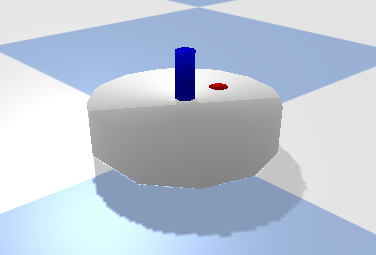
\includegraphics[width=0.8\textwidth]{figures/point_robot.png}
    \caption{The holonomic point robot the 2 velocity\\inputs drive the robot in \gls{x} and in \gls{y} direction}%
    \label{subfig:example_point_robot}
    \end{subfigure}%
    \begin{subfigure}{.5\textwidth}
    \centering
    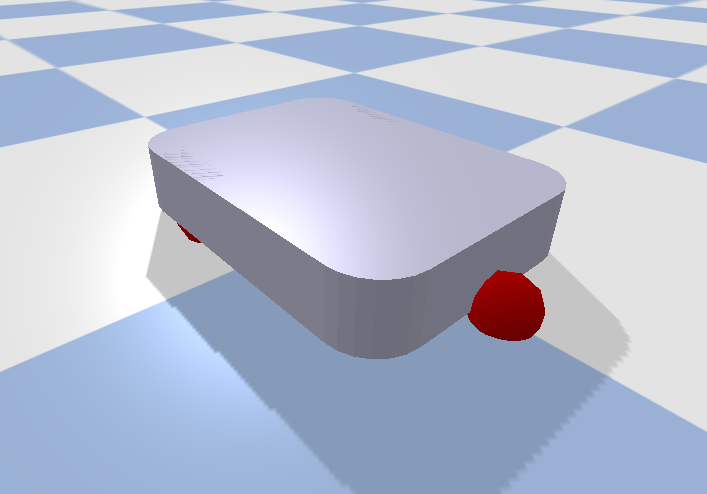
\includegraphics[width=0.8\textwidth]{figures/boxer_robot.png}
    \caption{The nonholonomic boxer robot, the\\first velocity input drives the robot forward\\ or backward the second rotates the robot}%
    \label{subfig:example_boxer_robot}
    \end{subfigure}%
    \caption{Robots used for testing the proposed method}%
    \label{fig:example_robots}
\end{figure}

\begin{figure}[H]
    \centering
    \begin{subfigure}{.5\textwidth}
    \centering
    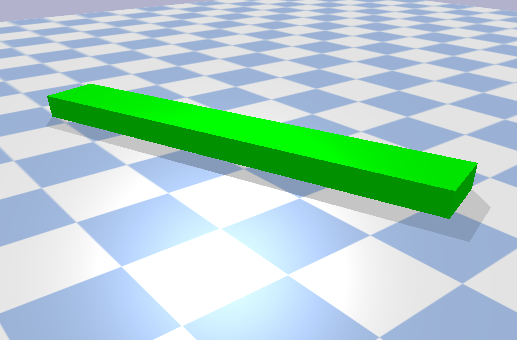
\includegraphics[width=0.8\textwidth]{figures/box_object.png}
    \caption{A box object}
    \end{subfigure}%
    \begin{subfigure}{.5\textwidth}
    \centering
    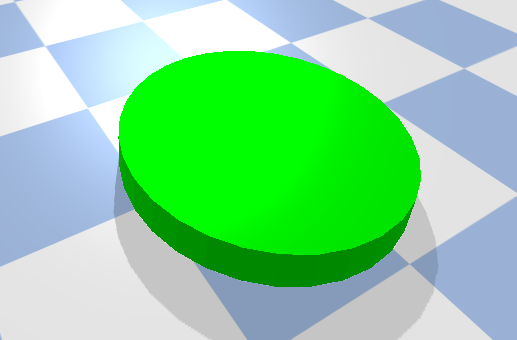
\includegraphics[width=0.8\textwidth]{figures/cylinder_object.png}
    \caption{A cylinder object}
    \end{subfigure}%
    \caption{Various objects in the robot environment}%
    \label{fig:example_objects}
\end{figure}

For complete environments with accompanying tasks, see~\Cref{chap:results}.\bs

\section{Report Structure}%
\label{sec:report_structure}
The proposed method heavily relies on a number of methods and functions. These methods and functions are conveniently grouped in \Cref{chap:required_background}. Then the proposed method is presented and discussed in \Cref{chap:hgraph_and_kgraph}. The proposed method is followed by a chapter committed to testing the proposed method, presented in \Cref{chap:results}. The last chapter dedicates itself to drawing conclusions on tests and answering the research questions in \Cref{chap:conclusion}.\bs
